\pagestyle{plain} % No headers, just page numbers
% \pagenumbering{arabic} % Arabic numerals
% \setcounter{page}{1}


\chapter{\uppercase {Multimodal Contextual Dialog Breakdown Detection for Conversational AI Models}}

Dialog breakdown detection is important in industry settings because it allows the system to correct for mistakes in real time. Real word conversational agents often use an ASR to convert the spoken instructions into text. Occasionally, the ASR model could miss some transcripts or have very noisy transcripts, especially when the user is in a setting with a lot of background noise or using a phone line with a poor network. With dialog breakdown detection, it is possible to detect that there was likely some missing context and respond with a generic message such as, “Sorry I missed that, could you repeat yourself?” to get the conversation back on track.

\begin{figure}
    \centering
    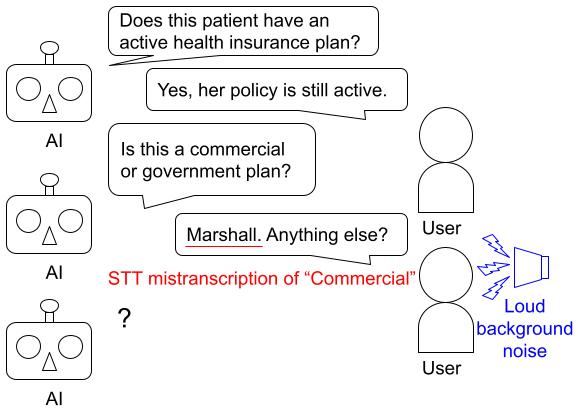
\includegraphics[width=3in]{images/db_example.jpg}
    \caption{Dialog breakdown in a phone conversation caused by loud noise from user end.
    }
    \label{fig:dialogue_breakdown_example}
\end{figure}

Dialog breakdown detection has some unique challenges in industry settings. In professional settings, people do not use as much explicit language or profanities. Hence, we often need to rely more on tone or cadence to detect user frustration. Additionally, there is a low tolerance for incorrect responses. For example, in the healthcare domain, a failed conversation could affect the time it takes for a patient to receive treatment. Finally, a lot of conversational agents have very complex and varied flows. For example, the average conversation in our domain consists of $\sim$ 100 turns, and context from early in the conversation can affect the flow even at the end of the conversation. 

There are additional challenges for detecting dialog breakdown in phone call settings. Over the phone, there are strict latency requirements (e.g. delayed or repeatedly incorrect responses can cause frustration or even hang-ups from users interacting with the system). In contrast, text-based chatbot systems often have visual feedback to indicate processing time and often target users and use cases with more leniency around latency and potential hallucinations. Thus, detecting dialog breakdowns in a timely manner is crucial for real-time conversational speech AI systems. It is an extremely challenging task because there are multimodal factors in different components of the system pipeline  which can appear as diverse downstream issues. 

We found that prior state-of-the-art models were not able to accurately capture dialog breakdown in our industry setting. In this work, we propose a new model that uses audio and text signals to predict dialog breakdown, generalizable to various industry use cases.

\section{Dataset}
We collected our data from calls driven by a conversational AI agent to verify the insurance benefits of patients for covering target medications. For our dialog breakdown detection model training and testing, we used 1,689 phone call conversations between the AI agent and users (e.g., insurance company employees) in which human intervention was required due to dialog breakdowns (e.g., AI agent misclassified intent due to mistranscribed STT caused by the high level of noise during the phone calls) from August 2023. More specifically for our objective of benefit verification calls, human intervention is required when 1) AI agents do not follow standard operating procedures as in the task definition and diverge from correct paths of conversations, 2) users get frustrated during the interaction. Reasons of frustrations can include repeated noncritical mistakes or slow responses of AI agents. 3) AI agents make critical mistakes, which may cause call failures immediately or in the later phase of the calls.  We used 70\% for training, 20\% for validation, and 10\% for testing for our model experiments. Then, we additionally collected 94 calls from September 2023 to test the generalizability of our best model (Table~\ref{tab:dataset}). Each phone call contains 104 to 112 turns on average between AI agents and users. The calls are randomly sampled to minimize any potential sampling bias towards specific gender, age or ethnicity of users. Binary labels of `breakdown' (turns for which human intervention was required) and `no breakdown' (turns with coherent conversation flows) are used for our dialog breakdown detection tasks.

\begin{table}
\small
\centering
\begin{tabular}{l|l|lll}
\hline
\textbf{Dataset Type} & \textbf{Calls} & \textbf{Turns} & \textbf{AVG} & \textbf{STDV}\\
\hline
Train & 1,181 & 124,384  & 105.32  & 28.34 \\ 
Validation & 338 & 35,985  & 106.46 & 28.33 \\ 
Test & 170 & 17,690 & 104.06 & 27.63 \\
Generalizability & 94 & 10,505 & 111.75 & 34.45 \\\hline 
\end{tabular}
\caption{\label{tab:dataset} Phone call dialog breakdown dataset. `AVG' column is the average number of turns for each call in the corresponding dataset, and `STDV' column is the standard deviation of turns for each call.}
\end{table}

\section{Methods}
\subsection{Baseline Models}

We explored potential methods, including the state-of-the-art models for text-only dialog breakdown detection. For baseline, we replicated the approaches that obtained the state-of-the-art performances from the previous work: LSTM and BERT \cite{sugiyama2021dialogue}. We implemented 4 dialog breakdown detection models that can leverage transcribed texts, and several available signals such as speaker information, intent classification of our AI model agent and raw audio signal. 

\begin{figure}
    \centering
    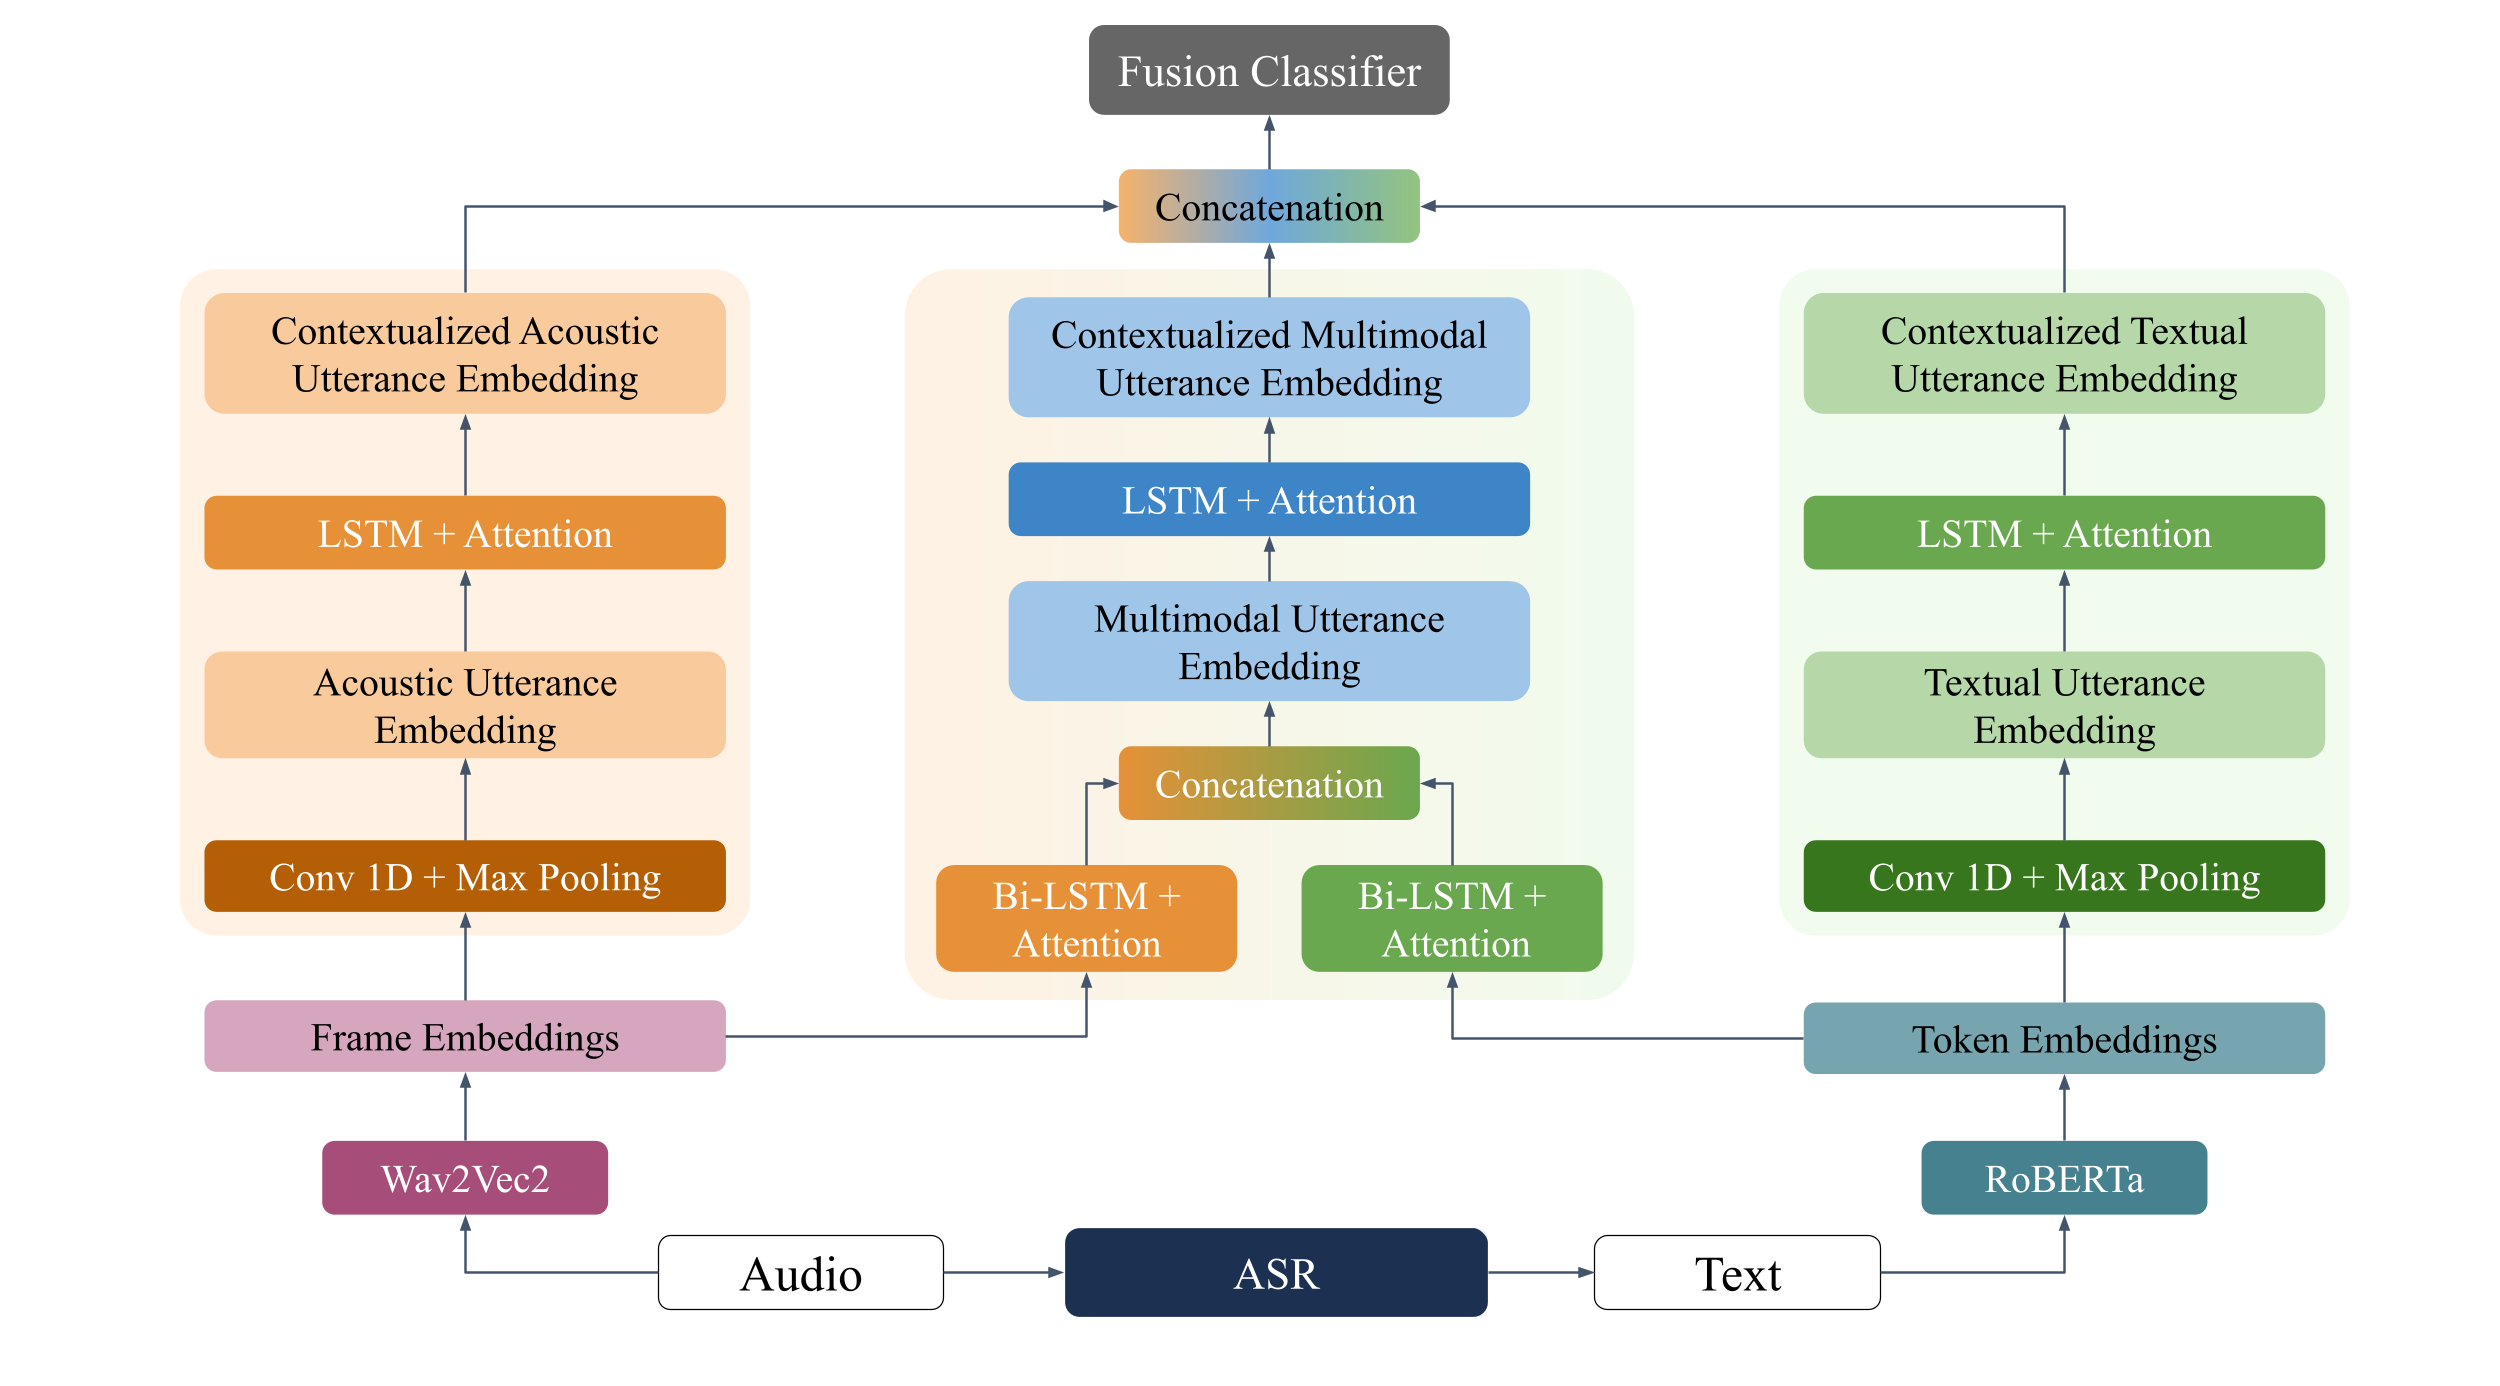
\includegraphics[width=6.5in]{images/db_updated_model_diagram.png}
    \caption{MultConDB model architecture. 
    }\label{fig:multimodal_lstm}
\end{figure}



\textbf{Text LSTM}: \label{lstm}
In this model, we have extended the work of \cite{Hendriksen2021}, which utilizes pre-trained GloVe embeddings to model utterance representations and uses different variants of LSTM to detect dialog breakdown~\cite{pennington2014glove}.
In our implementation, we have extracted contextualized token embeddings using pre-trained RoBERTa \cite{liu2019roberta} model instead of non-contextualized GloVe embeddings. The choice of embedding is inspired by the recent surge of Transformer \cite{NIPS2017_3f5ee243} based embeddings in the literature, where they are proven to yield better performance than non-contextualized GloVe embeddings. While \cite{Hendriksen2021} generates utterance embeddings by averaging all the word embeddings in an utterance, we employ a Bi-LSTM layer and attention to further process and combine the RoBERTa-based token embeddings into the utterance embedding. We have employed another layer of Bi-LSTM and attention to accumulate contexts from the current and all previous utterance embeddings. The contextualized utterance embedding is then passed through a linear classifier layer, which classifies each utterance into either the breakdown or the non-breakdown class.  

\textbf{End-to-End LLM Classifier}: In the previous Text LSTM model, we used an LLM, RoBERTa, as a feature extractor for extracting the token embeddings in the input utterances, but we did not use the RoBERTa model in end-to-end settings. To leverage the full capabilities of an LLM, in this LLM model, we finetune the RoBERTa-base model with a classification head on top to classify the input utterance into breakdown or non-breakdown classes. In this implementation, we get rid of additional Bi-LSTM and attention networks for contextualization as we incorporate contextual information as the input to the model. Similar to the previous model, each utterance is represented as a concatenation of the speaker tag, utterance text and intent. The linear layer and the layers of RoBERTa-base model are fine-tuned end-to-end. We have experimented with different configurations of the linear layers and based on the empirical results, we use 2 linear layers with 784 and 2 neurons each and the latter works as a classification layer.  

\textbf{Multimodal Transformer (MulT A+T)}: 
\cite{tsai-etal-2019-multimodal} introduced the Multimodal Transformer model for emotion recognition, which leverages the transformer architecture and cross-modal attention mechanisms. This model serves as a popular baseline for emotion recognition tasks. In our research, we have adapted this model to suit the specific task of dialog breakdown detection. The original implementation of the Multimodal Transformer incorporated three modalities (audio, video, and text), but we focus on using audio and ASR-generated text and used positional encodings to enhance the model's understanding of positional information. 

The core component of our model is the cross-modal transformer, which facilitates the integration of information from both audio and text. In the first transformer block, acoustic inputs are used as queries, while textual inputs serve as both keys and values. In the second block, these roles are reversed, with textual inputs as queries and acoustic inputs as keys and values. This approach enables effective cross-modal information exchange through attention mechanisms. Within the cross-modal transformer blocks, we employ a stack of 12 cross-modal attention layers (4 attention heads per layer). Then, the outputs are passed through traditional self-attention-based transformers (6 attention layers and 4 attention heads per layer). Following this, we apply pooling operations to the outputs from both transformer blocks and concatenate them. This concatenated representation is then passed through a series of linear layers for classification. Our architecture includes two projection layers and one classification layer. 

\subsection{MultConDB}
We introduce a model named \textbf{Mult}imodal \textbf{Con}textual \textbf{D}ialogue \textbf{B}reakdown detection, or MultConDB, which is inspired by and built upon the model proposed by \cite{miah-etal-2023-hierarchical} in their work on hierarchical online dialog act classification. Our model consists of two unimodal encoder branches and one multimodal encoder branch. The unimodal encoder branches individually handle textual and acoustic features, producing two distinct unimodal encodings: one for acoustic data and one for textual data. We used Wav2Vec2~\cite{10.5555/3495724.3496768} as our acoustic feature extractor. We standardize every user or AI agent utterance by converting it into 15 second chunks through padding or trimming and subsequently extract frame-level features using Wav2Vec2, with each frame having a duration of 25 ms and a stride of 20 ms. For textual data, Token-level features are extracted in a similar manner, utilizing RoBERTa as described in `Text LSTM'.

These unimodal encoder branches share an identical architecture. Initially, frame-level or token-level features undergo processing via temporal convolutional layers, each equipped with 256 kernels (size = 5). This temporal convolution operation contextualizes the frames. Following temporal convolution, we apply a max-pooling operation to generate a single embedding vector for each utterance. We pass these utterance embeddings through an LSTM and an attention network to incorporate contextual information from a set of previous utterances. This process yields both acoustic and textual utterance embeddings.

In the multimodal branch, we employ two Bi-LSTMs along with an attention network to separately process token embeddings and frame embeddings. This approach results in a pair of utterance embeddings derived from textual and acoustic features. These embeddings are concatenated to create a multimodal embedding at the utterance level. To further enrich contextual understanding, we introduce another layer of LSTM and an attention network, taking into account context from both the current and past utterances. We empirically determine the optimal attention window size to be 5. Subsequently, we concatenate the two unimodal and one multimodal contextualized utterance embeddings to form a fusion embedding. This fusion embedding undergoes further processing through linear layers, consisting of 256 neurons and 2 neurons. Finally, the last linear layer classifies whether each input utterance is a dialog breakdown.


\section{Results and Analysis}

\subsection{Task Evaluation \label{sec:task_eval}}
\begin{table}
\small
\centering
\begin{tabular}{l|l|lll}
\hline
\textbf{Model} & \textbf{Inputs} & \textbf{Prec} & \textbf{Rec} & \textbf{F1}\\
\hline
Text LSTM & S+U+I & 39.78 & 65.30 & 49.44 \\ 
End-to-End LLM & S+U+I & 64.03 & 52.35 & 57.61 \\ 
MulT A+T & S+U+I+A & 63.51 & 55.29 & 59.12 \\\hline
MultConDB & S+U+I+A  & \textbf{65.96} & \textbf{72.94} & \textbf{69.27} \\\hline
\end{tabular}
\caption{\label{tab:model_performance} Model performance for dialog breakdown detection. Columns are defined as `Inputs': types of inputs, `Prec': precision, `Rec': recall and `F1':dialog breakdown prediction F1 score. Each row of `Input' column values are defined as following: `S': speaker tag (\textit{AI agent} or \textit{User}), `U': utterance, `I': intent prediction of \textit{AI agent model}, `A': audio recording of utterances.}

\end{table}

\textbf{Dialog Breakdown Performance Analysis:} We evaluated the models in our dialog breakdown dataset collected from August 2023 (Table~\ref{tab:dataset}). We conducted hyperparameter tuning of each model architecture using the validation set (random 20\% of the August calls) and trained with our training set (random 70\% of August calls). Each model took speaker tags, utterances, AI agent model intents of the current turn, and historical turns within its context window as input and predicted whether the current turn is a dialog breakdown. We reported their performances on the test set (random 10\% of August calls). We conducted fine-tuning and hyperparameter tuning of each model on the August validation set.

For preliminary analysis, we used plain texts without intents predicted by our conversational AI model agent for each model architecture and in-context learning (ICL) approaches~\cite{brown2020language} with Gemini Pro and the best F1 was 40.31 (see more details in Section~\ref{sec:prelim}). This result suggested that it might be difficult to capture phone call dialog breakdowns within a few shots without audio context, such as noise or intonation, or the voice tones of users. Thus, we first explored text-based models by fine-tuning and training with dialog breakdown turns as labels so they can leverage the full training dataset (`Text LSTM' and `End-to-End LLM'). Then, we trained multimodal models with both acoustic and text signals (`MulT A+T' and `MultConDB').

In general, multimodal models obtained higher F1 scores than text-only models. This trend suggests that multimodal settings leveraging both text and audio signals are more effective for capturing phone call dialog breakdowns. Among Multimodal models, MultConDB obtained the best F1 score for classifying dialog breakdowns, 15\% F1 score improvement over Multimodal Transformer (p < 0.001). This may indicate that multimodal contextual model architecture and training process designed specifically for detecting dialog breakdown are critical to obtain the performance level of practical use.

\begin{figure}
    \centering
    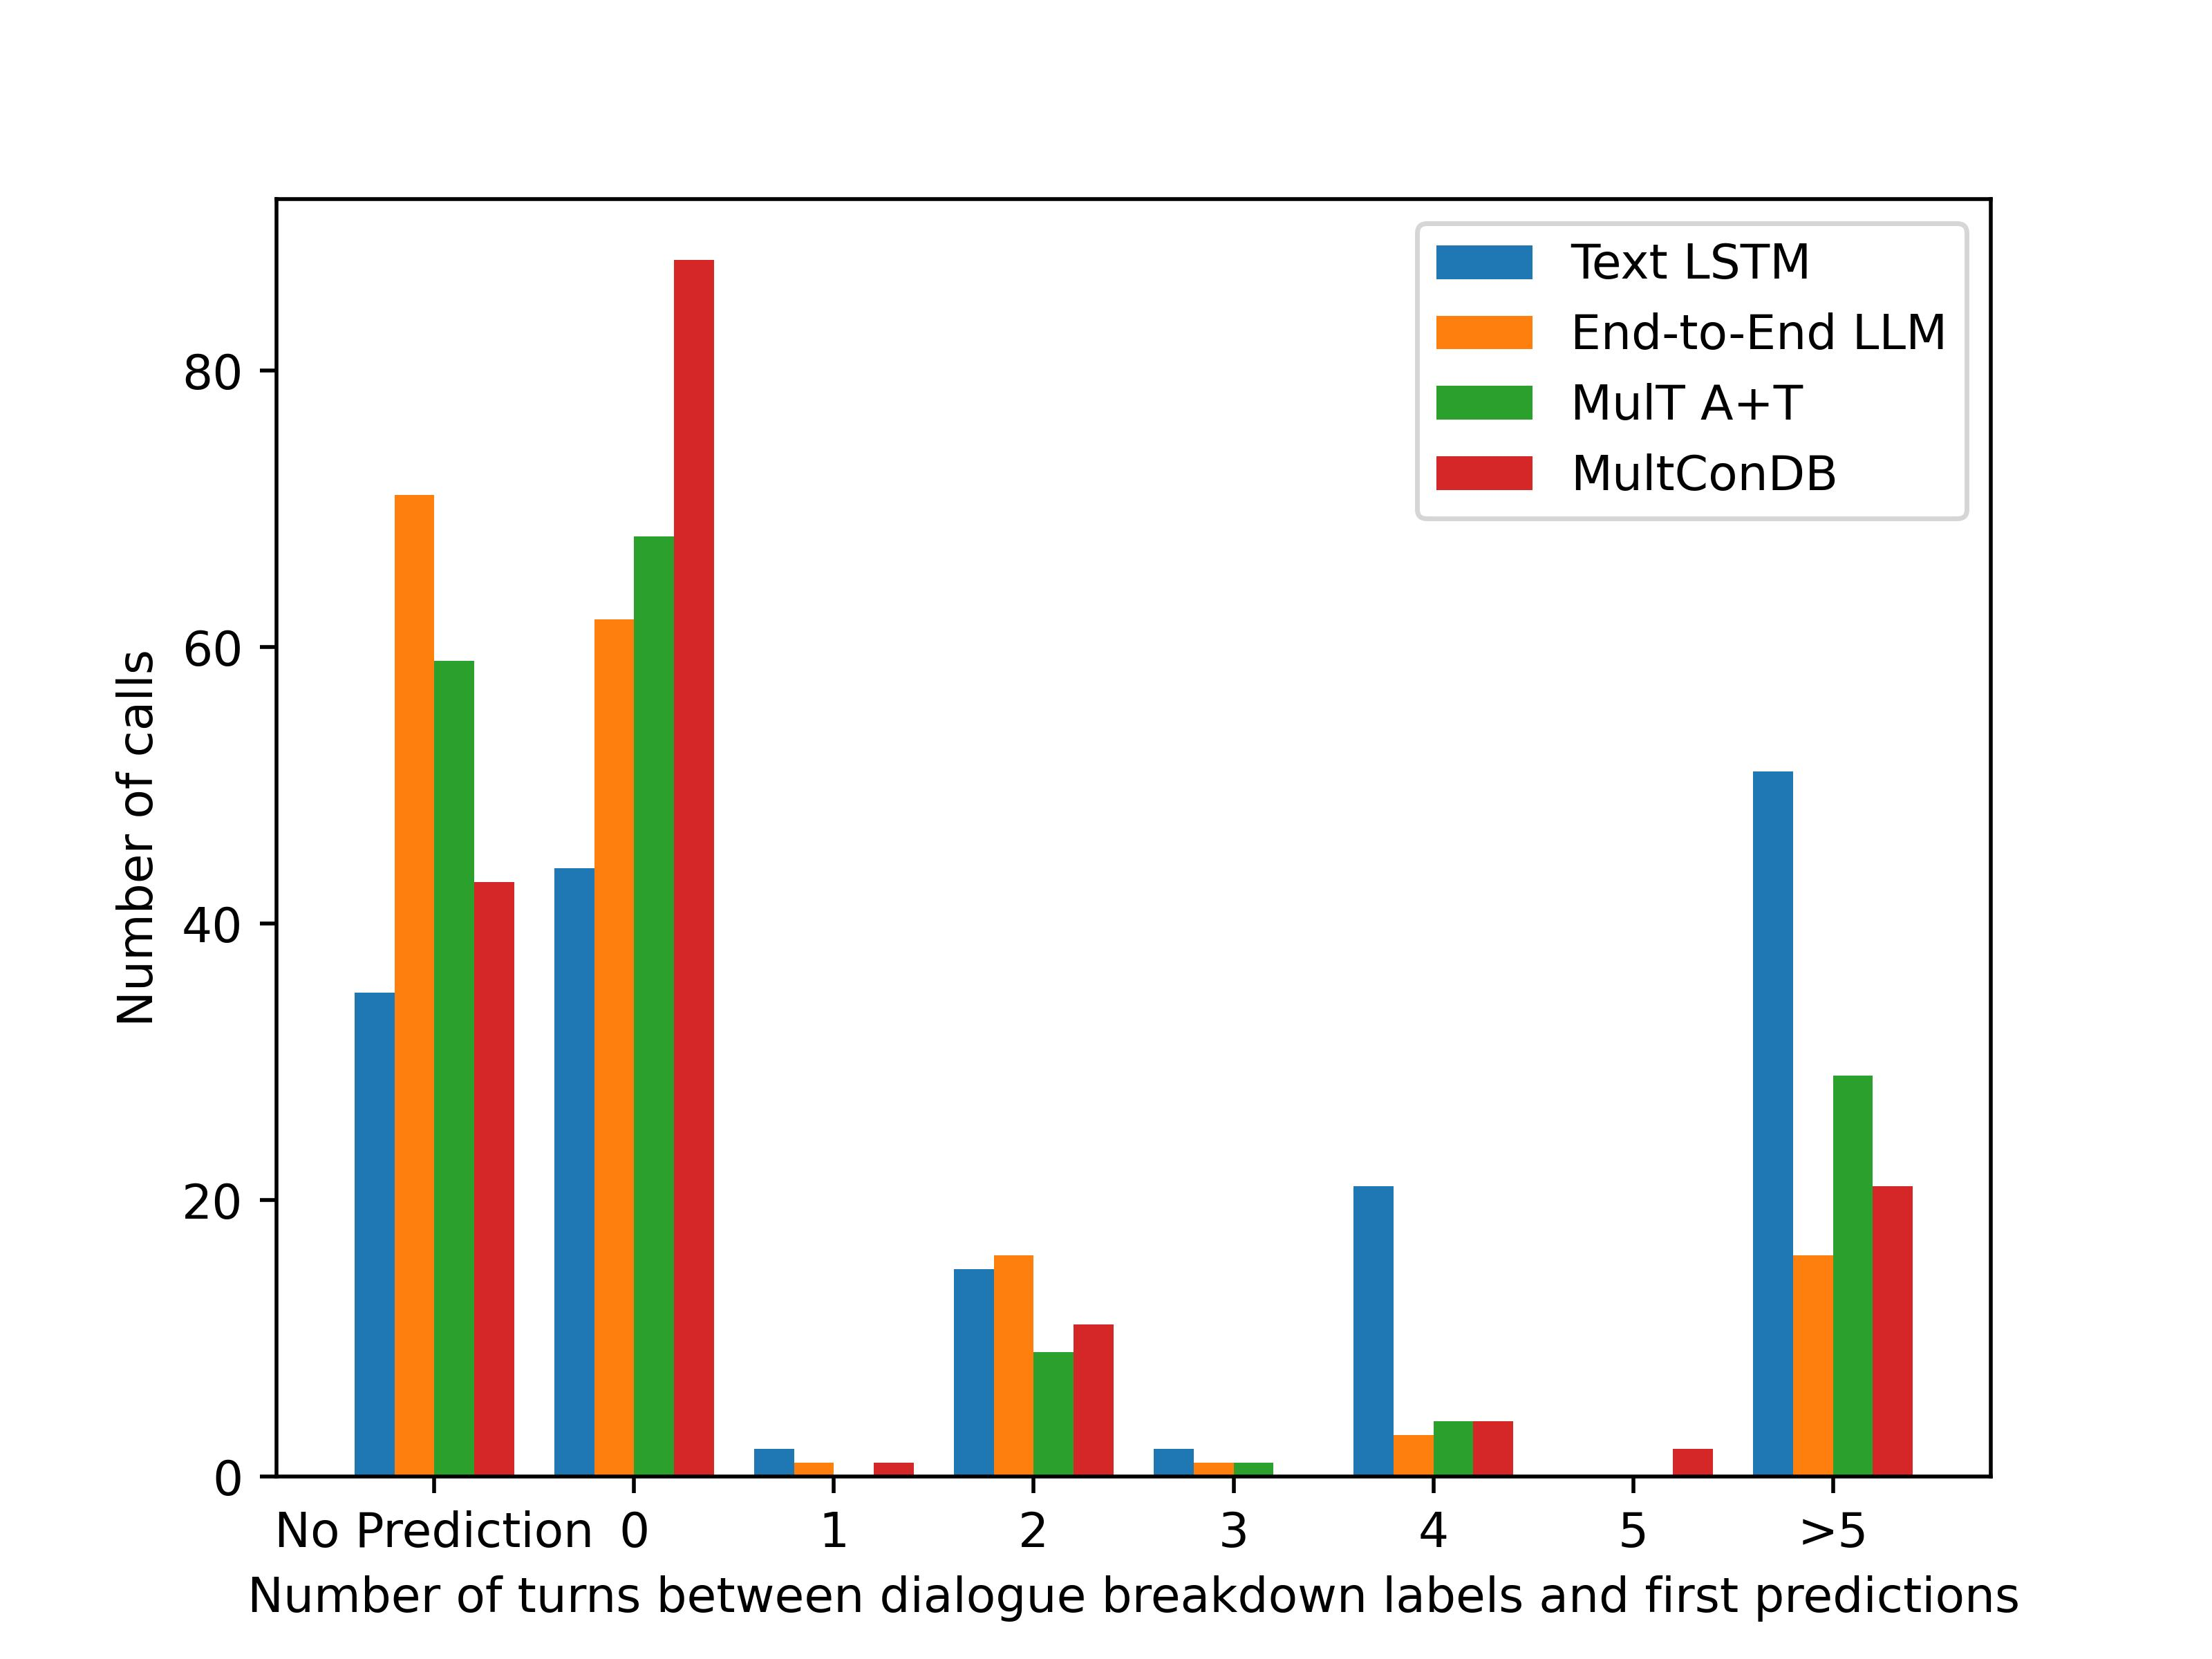
\includegraphics[width=4in]{images/db_Turns_Between_Labels_and_First_Predictions.jpg}
    \caption{Number of turns between dialog breakdown ground truth and first model predictions.}
    \label{fig:false_positive_analysis}
\end{figure}

\textbf{False Positive Analysis:} In addition to detecting exact dialog breakdown turns, it is also important for models to make false positive dialog breakdown predictions as near as possible to the actual breakdown point, if any. In industry settings in which large-scale automated phone calls happen concurrently, the dialog breakdown detection model should bring human in the loop near the breakdown points; otherwise, human feedback at the false positive turns is not useful as well, and overall call failure rates may increase because other phone calls with actual dialog breakdown may not get support from human intervention in time.

In Figure~\ref{fig:false_positive_analysis}, we measured the number of turns between the dialog breakdown turns and the first dialog breakdown predictions of the models. Multimodal models tend to make dialog breakdown predictions in nearer turns to breakdowns than text-only models do. This difference might have been caused by audio context, which can provide noise or speech timing of user and the  AI agent, which might cause dialog breakdown in the near future. Although End-to-End LLM had the smallest number of false positives more than 5 turns away from the breakdown points, it has the largest number of false negatives (`No prediction' in Figure~\ref{fig:false_positive_analysis}) and this trend can increase overall dialog breakdown detection failure rates. MultConDB obtained the highest of true positive predictions and the second lowest number of false positives, more than 5 turns away, and false negatives following the extremely high precision model (End-to-End LLM) and high recall model (Text LSTM), respectively.



\begin{figure}
    \centering
    \includegraphics[width=4in]{images/db_MultConDB_Before_and_After.jpg}
    \caption{Breakdown and non-breakdown turns of users and our conversational AI model captured by our model output layer. \textit{Before} figure shows 2D t-SNE of our model input embedding (concatenation of speaker tag, utterance, AI agent intent and audio) and \textit{After} figure shows the last output layer of our model right before prediction head softmax layer.
    }
    \label{fig:model_output_layer_analysis}
\end{figure}

\subsection{MultConDB Qualitative Analysis}
We analyzed the efficacy of our dialog breakdown detection model in terms of whether our multimodal contextual model architecture is effective for capturing phone call dialog breakdowns. In Figure~\ref{fig:model_output_layer_analysis}, model inputs in \textit{Before} figure show that breakdown and non-breakdown turns are not linearly separable and difficult to classify without contextualization; they are spread around without any specific patterns. In contrast, our model outputs in \textit{After} suggest that our model architecture was quite effective for all types of dialog breakdown turns; breakdown turns are clustered on the right side of the figure. Dialog breakdown turns are difficult to capture because the same utterance text can be a dialog breakdown turn or a natural conversation flow turn based on the context and acoustic signals. Also, the same sentence can be a question, statement, or continuing speech with a short pause before the following statement based on its intonation and context so the response of our AI agent is likely to cause a dialog breakdown and provide a negative experience to users if it interrupts users' speech, or it goes silent when it misunderstands a question as a statement. This analysis suggests that  MultConDB can classify dialog breakdown utterances leveraging these types of subtle nuances and contexts. 


\subsection{Underlying Causes of Breakdowns}

\begin{figure}
    \centering 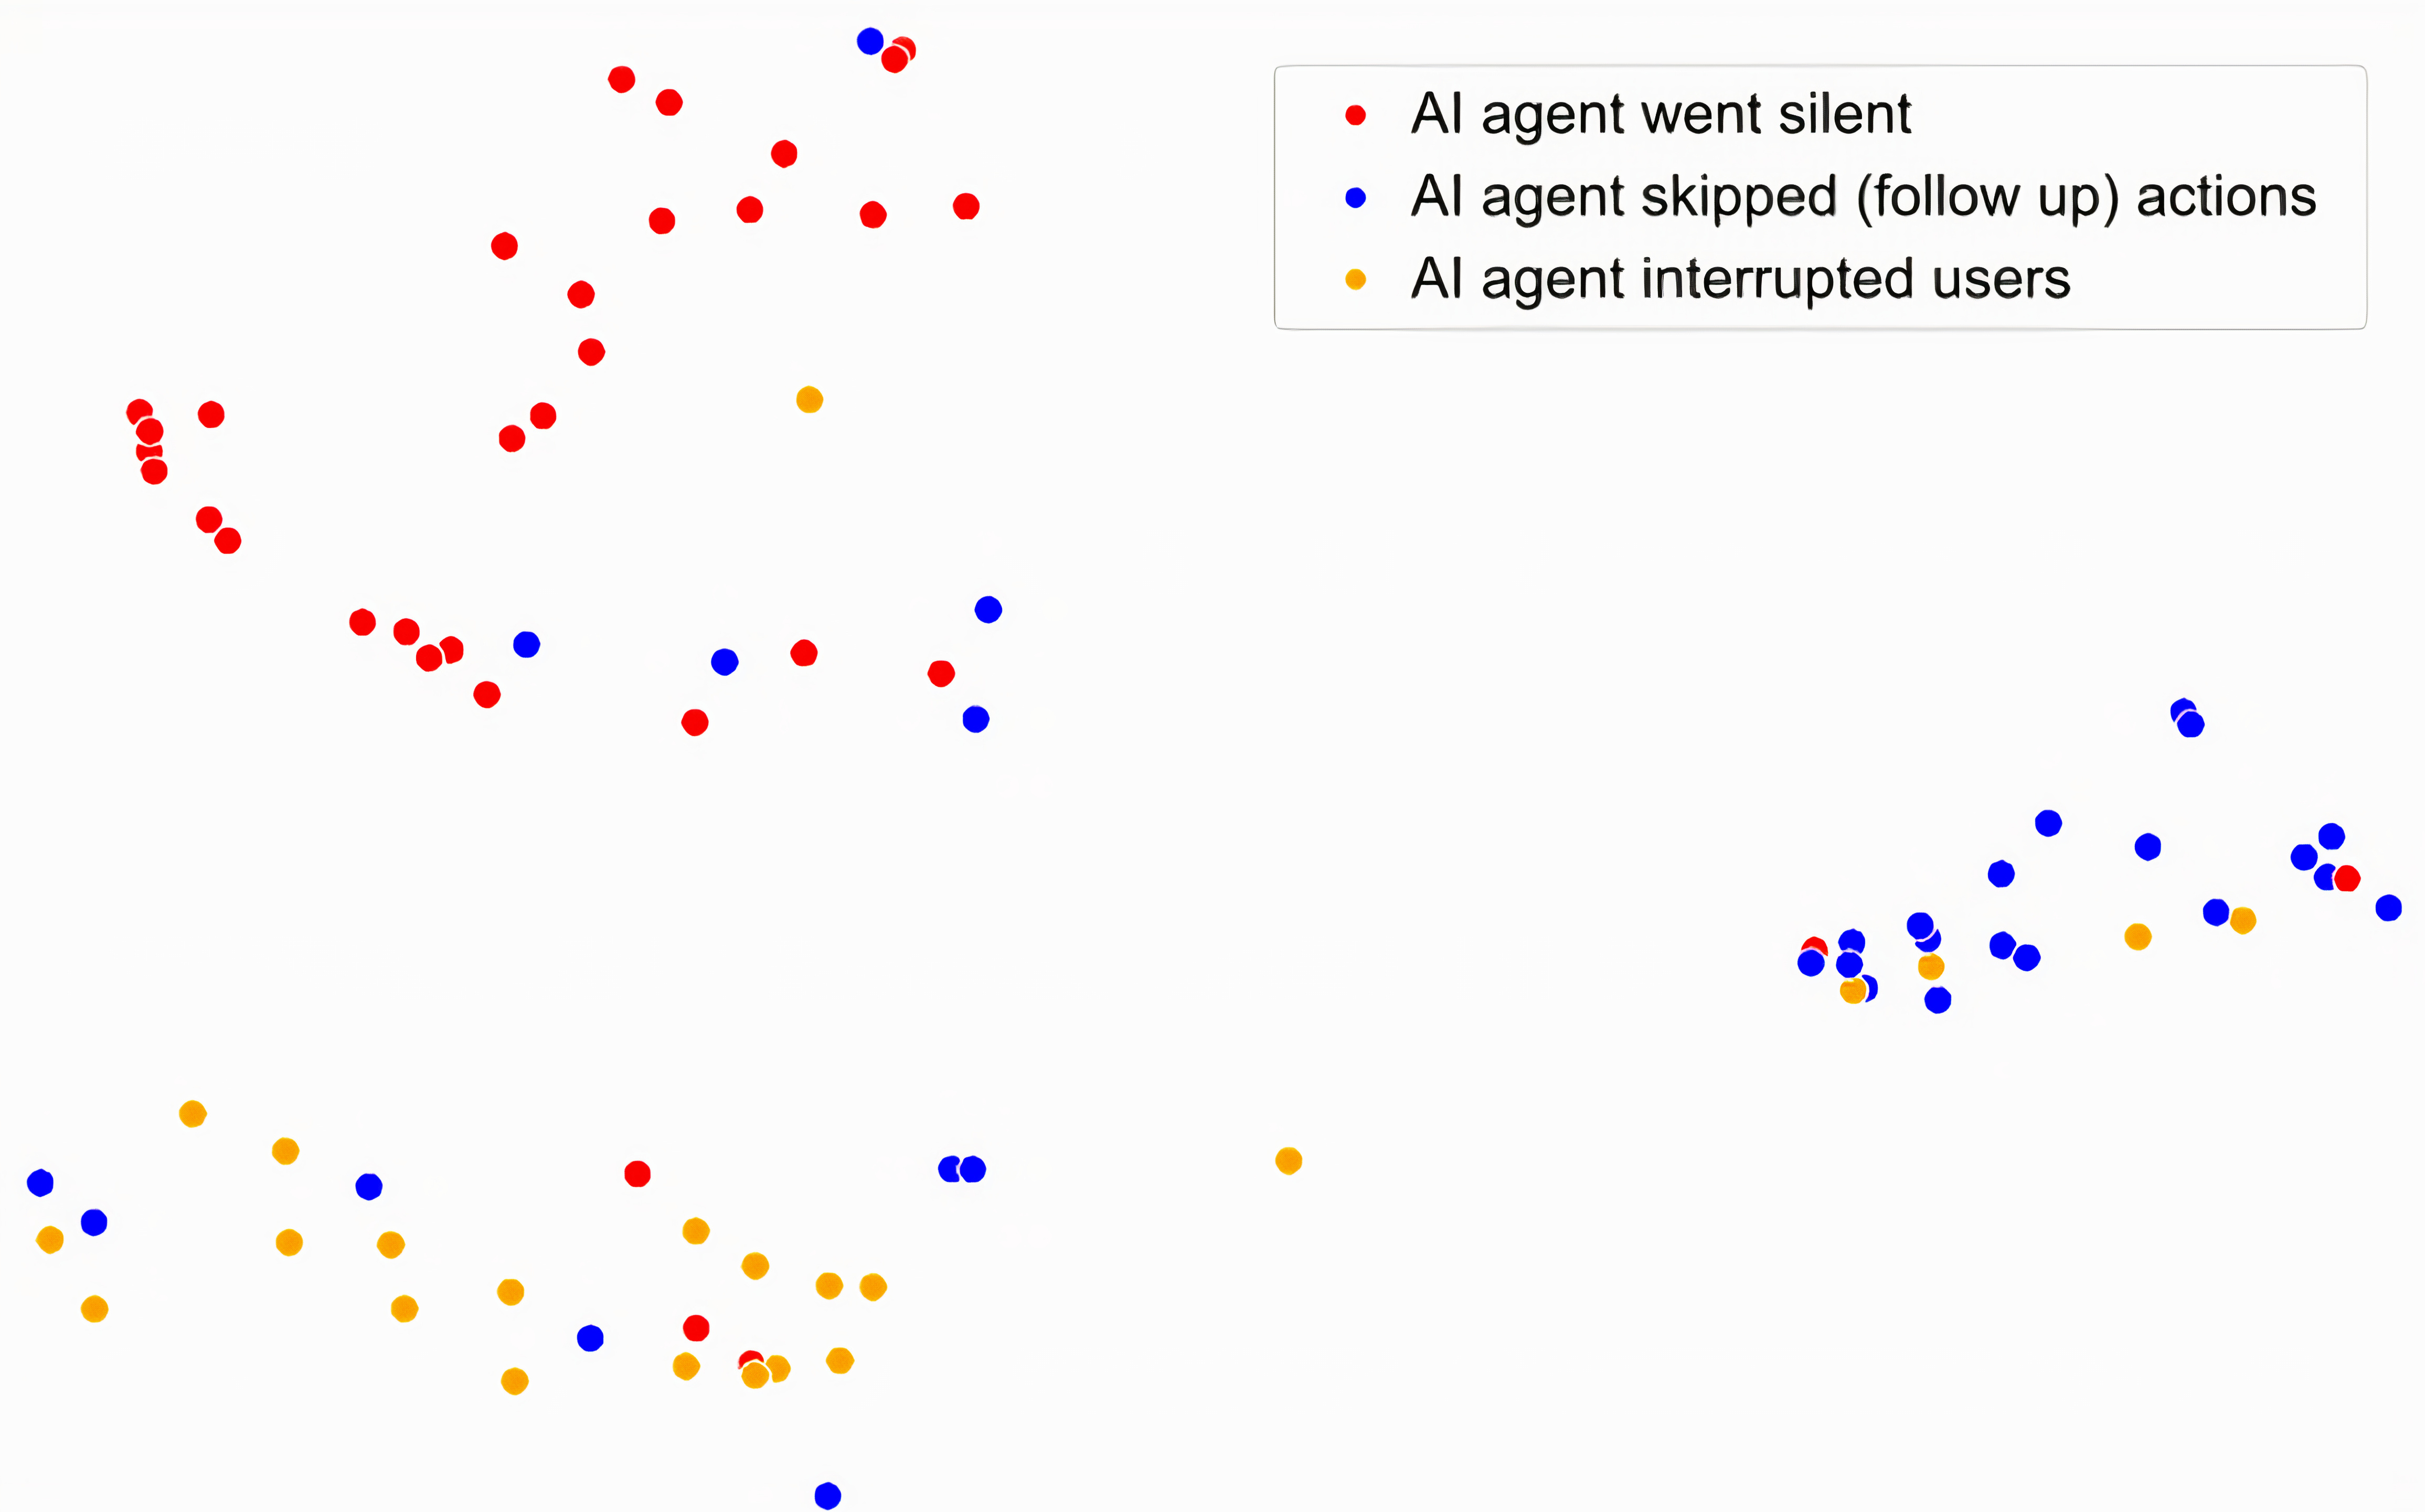
\includegraphics[width=4in]{images/db_MultConDB_Dialogue_Breakdown_Types_Embedding_Analysis.jpg}
    \caption{2D t-SNE of MultConDB output layers colored by types of dialog breakdown.}
    \label{fig:3_error_categorization}
\end{figure}

For additional analysis to validate whether MultConDB is effective for inherently categorizing types of dialog breakdowns further, we conducted a visualization analysis for MultConDB output layers for its capability of categorizing the causes of dialog breakdown. Among dialog breakdown utterances in our testset phone calls, we identified the most distinguishable and clear causes of dialog breakdowns as follows: \textbf{AI agent went silent} (34 turns). For example, (1) AI agent may wait for responses when it misclassifies the end of speech from users as continuing speech or upstream STT finalization was delayed, (2) \textbf{AI agent interrupted users} (23 turns). For example, AI agent may misclassify continuing speech of users as the end of speech and ask the next question while the users are providing their answers, and (3) \textbf{AI agent skipped required actions or follow-up actions} (31 turns). For example, loud noises can cause a high rate of STT mistranscriptions, which cause intent misclassification of the  AI agent. 
Although we have not trained MultConDB with explicit labels of types of dialog breakdown, it inherently captured which type of underlying causes led to dialog breakdown. In Figure~\ref{fig:3_error_categorization}, the turns after which the AI agent went silent were clustered on the top left, and the turns in which the AI agent interrupted the speech of users were clustered on the bottom left. Finally, the turns where the AI agent skipped required actions or follow-up actions were clustered on the right side. This suggests that MultConDB can capture abnormal conversation flows based on acoustic and text contexts, such as the voices of AI agents and users being combined in one turn\footnote{Potential acoustic signals of AI agents interrupting users.} or an AI agent not following up after the question intonation of users' speech, breaking the alternating turns of each voice.

\subsection{Dialog Breakdown Detection Model Generalizability Testing} \label{sec:generalizability_main}

In real-world industry settings, dialog flow and utterance distributions in phone calls keep changing everyday because outbound call target users have different call volumes everyday and they may ask different types of questions based on their policy changes. Also, the conversational AI agent models are maintained and updated with new releases. Thus, it is critical for the dialog breakdown models to generalize effectively to various types of dialog flows and interactions which have not been observed during its training process. 

To that end, we tested our dialog detection model on unseen data. We used 94 calls from September 2023 (Table~\ref{tab:dataset}) which include calls driven by updated AI agent models with new releases to validate how well MultConDB can generalize to unseen calls. MultConDB obtained F1 score 71.22 with precision 65.77 and recall 77.66 maintaining a high performance. In Figure~\ref{fig:generalizability}, it had an almost similar pattern to its prediction pattern from its August 2023 call data although the model is used for classifying dialog breakdown calls in a different month. Even though it had a relatively high number of false positive predictions more than 5 turns away from the actual dialog breakdown differently from the call data August, it still had the largest number of true positive predictions (0 in the figure) followed by no prediction as the second highest number of prediction category. These results suggest that MultConDB was not biased towards the types of dialog breakdowns caused by the previous release version of AI agent model and it can generalize well to other types of dialog breakdowns including the in correct reponses or abnormal conversation flows caused by the updated version of AI agent model or potentially other types of context introduced in a different month. 

\begin{figure}
    \centering 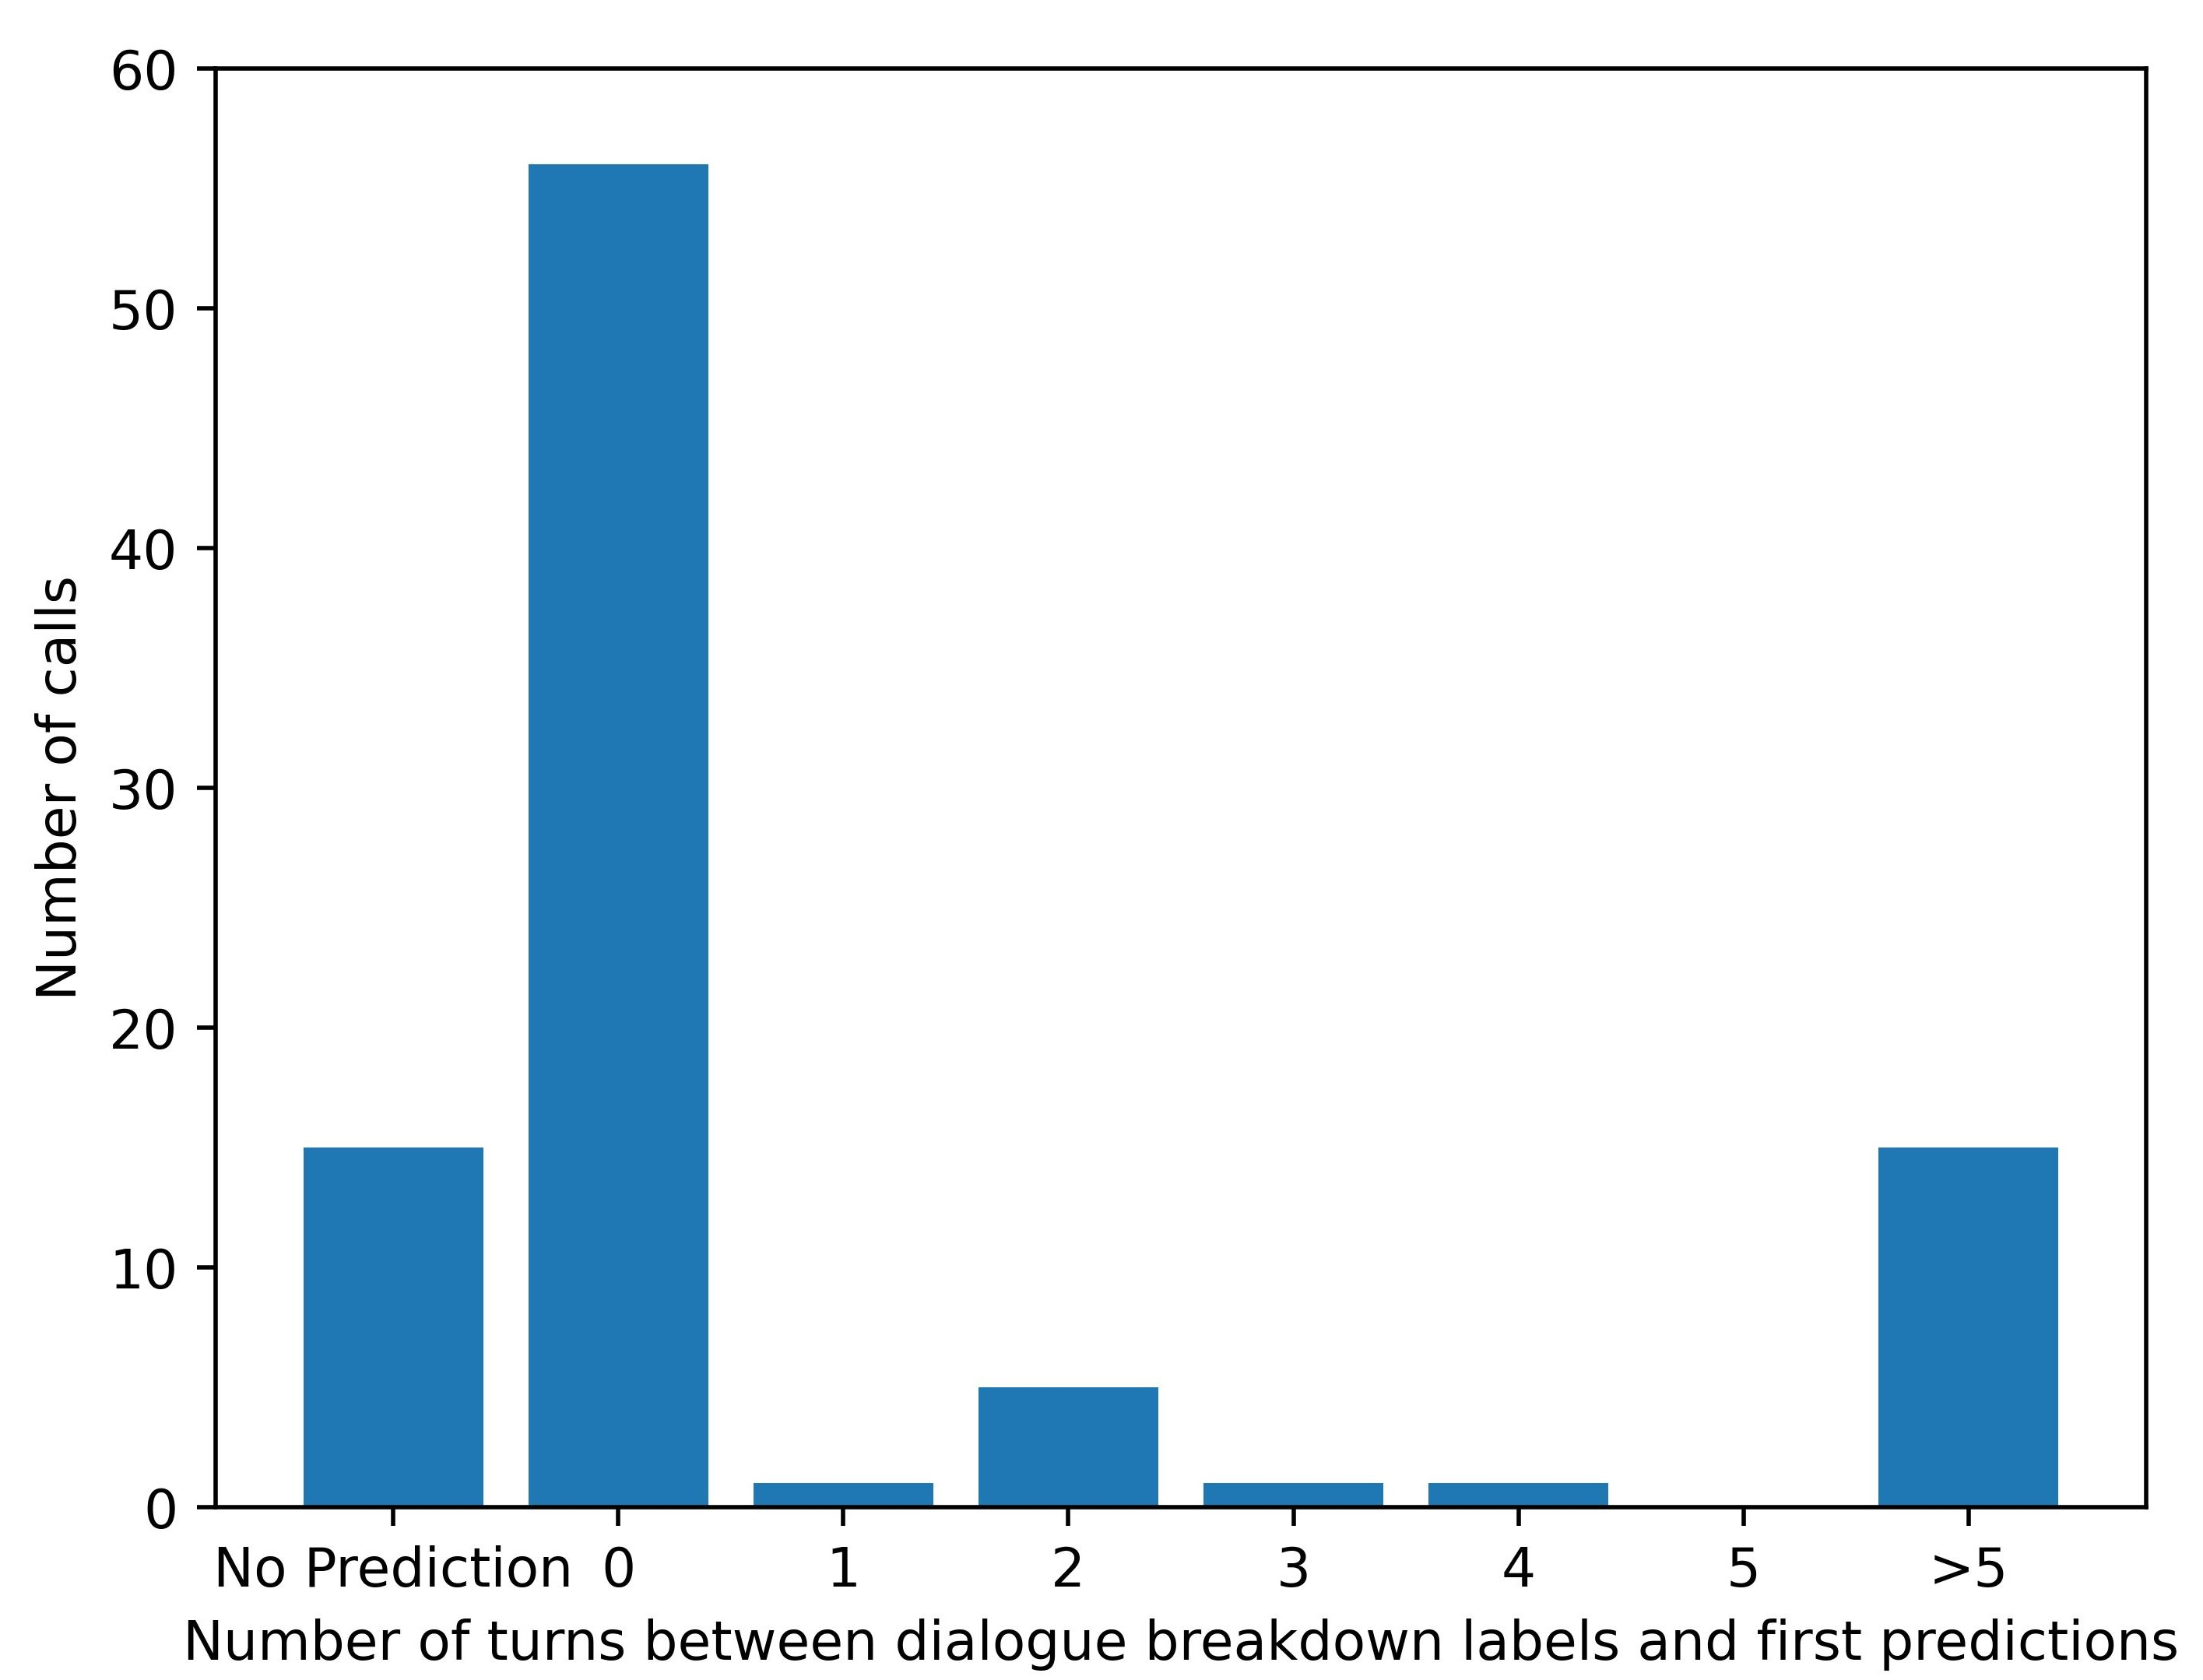
\includegraphics[width=4in]{images/db_Turns_Generalizability_Testing_cropped.jpg}
    \caption{Number of turns between dialog breakdown
ground truth and first model predictions in September 2023 calls.}
    \label{fig:generalizability}
\end{figure}

\section{Summary}
As the first work of multimodal dialog breakdown detection in healthcare industry settings, we explored various approaches leveraging both audio and text and developed a high-performance multimodal model (F1 = 69.27), which generalized well to various types of context of conversations driven by conversational AI models across multiple version releases in industry settings. Additionally, we conducted a thorough qualitative model analysis, which provided insights into its output patterns that can cluster dialog breakdown samples and their categories in separate groups.